\documentclass[11pt,a4paper]{article}

% --- Packages ---
\usepackage[utf8]{inputenc}
\usepackage[LGR,T1]{fontenc}
\usepackage{lmodern}
\usepackage[greek,english]{babel}
\usepackage{csquotes}
\usepackage{microtype}
\usepackage{geometry}
\geometry{margin=2.5cm}

\usepackage{amsmath,amssymb}
\usepackage{graphicx}
\usepackage{booktabs}
\usepackage{hyperref}
\hypersetup{
  colorlinks=true,
  linkcolor=blue!60!black,
  citecolor=blue!60!black,
  urlcolor=blue!60!black,
}
\usepackage{xcolor}
\usepackage{listings}
\usepackage{tikz}
\usetikzlibrary{arrows.meta,positioning,shapes.geometric,calc}

% Code listing style
\lstset{
  basicstyle=\ttfamily\small,
  breaklines=true,
  frame=single,
  framesep=3pt,
  xleftmargin=6pt,
  xrightmargin=6pt,
  backgroundcolor=\color{gray!5},
  rulecolor=\color{gray!40},
}

% Convenience macros
\newcommand{\crm}{\mbox{CIDOC-CRM}}
\newcommand{\crmrag}{\mbox{CRM-RAG}}
\newcommand{\prop}[1]{\texttt{#1}}
\newcommand{\cls}[1]{\texttt{#1}}
\newcommand{\fn}[1]{\texttt{#1}}

% --- Title ---
\title{\crmrag{}: A Graph-Aware Retrieval System\\for Cultural Heritage Knowledge Graphs}
\author{}
\date{}

\begin{document}
\maketitle

% ===================================================================
\begin{abstract}
Cultural heritage institutions increasingly publish their collections as structured knowledge graphs using the \crm{} ontology and~RDF\@.
While these representations are rich and interoperable, they are not amenable to direct natural language querying.
This article presents \crmrag{}, a retrieval-augmented generation system that bridges the gap between structured knowledge graphs and conversational question answering.
The system converts RDF data into entity-centric natural language documents through ontology-guided traversal, indexes them for hybrid dense--sparse retrieval, and applies graph-aware re-ranking to select contextually coherent document sets for answer generation.
We describe the architecture in detail, tracing the lifecycle of data from its origin as RDF triples through every transformation and storage layer to its final consumption at query time.
\end{abstract}

% ===================================================================
\section{Introduction}
\label{sec:intro}

Museums, archives, and cultural heritage institutions describe their collections through structured data.
An artwork has a creator, a creation date, a physical location, a material, and a depicted subject.
These facts are increasingly stored not as free text but as knowledge graphs---databases of precise, machine-readable statements that link entities to one another through typed relationships.
The adoption of shared ontologies such as \crm{} has made these graphs interoperable across institutions, enabling federated queries over collections that were previously siloed.

However, a persistent gap remains between the structured richness of these graphs and the natural language that researchers, curators, and the public use to ask questions.
A scholar studying Byzantine iconography in Cyprus wants to ask \enquote{Which saints are depicted in the frescoes of Panagia Phorbiottisa?}---not to write a multi-join SPARQL query that navigates through intermediate production events and visual representation nodes.
Retrieval-Augmented Generation (RAG) offers a promising approach to this problem, but standard RAG systems are designed for text corpora: articles, web pages, manuals.
They assume the knowledge source is already in document form.
A knowledge graph is not.

\crmrag{} addresses this mismatch.
It converts a \crm{} knowledge graph into a corpus of entity-centric natural language documents, where each document captures not only an entity's direct properties but also its multi-hop relationships discovered through ontology-guided path traversal.
These documents are then indexed for hybrid dense--sparse retrieval and re-ranked using a graph-aware selection algorithm that favors contextually connected document sets over isolated high-similarity results.

This article describes the system's architecture in full.
It assumes no prior familiarity with RDF, SPARQL, \crm{}, or machine learning, introducing each concept as it becomes relevant.
The presentation follows the flow of data through the system: from its origin as RDF triples in a SPARQL endpoint, through document generation and indexing, to its final consumption during question answering.

% ===================================================================
\section{Background}
\label{sec:background}

\subsection{Knowledge Graphs and RDF}
\label{sec:rdf}

A knowledge graph stores information as a collection of \emph{triples}---statements composed of exactly three parts: a subject, a predicate, and an object.
Each part is identified by a URI (Uniform Resource Identifier), a globally unique string that functions as a stable name for a real-world entity, relationship, or value.
A triple such as

\begin{lstlisting}
<http://example.org/church/panagia>
  <http://cidoc-crm.org/P55_has_current_location>
    <http://example.org/place/nikitari>
\end{lstlisting}

\noindent states that the church of Panagia Phorbiottisa has its current location at the Village of Nikitari.
The subject is the church, the predicate describes the nature of the relationship, and the object is the place.
A knowledge graph is simply a large collection of such triples.
Taken together, they form a directed labeled graph in which entities are nodes and relationships are edges.

RDF (Resource Description Framework) is the W3C standard for encoding triples.
It is used across museums, libraries, and cultural heritage institutions worldwide, and it is the representation assumed throughout this article.
SPARQL is the corresponding query language, analogous to SQL for relational databases.
A SPARQL query can retrieve all triples involving a given entity, all entities belonging to a given class, or any subgraph matching a specified pattern.

\subsection{CIDOC-CRM and Fundamental Relationships}
\label{sec:cidoc}

An ontology is a shared vocabulary for a domain---an agreed-upon set of classes and properties that standardize how things relate to each other.
Without an ontology, one museum might call a property \enquote{creator,} another \enquote{made\_by,} and a third \enquote{artist.}
An ontology ensures that all institutions use the same terms with the same semantics.

\crm{} (International Committee for Documentation---Conceptual Reference Model) is the ISO standard ontology for cultural heritage (ISO~21127)~\cite{leboeuf2023}.
It defines a class hierarchy for describing the entities that appear in cultural heritage data.
Physical objects such as paintings, sculptures, and churches are modeled as instances of \cls{E22\_Human-Made\_Object}.
People and organizations fall under \cls{E39\_Actor}.
Locations are \cls{E53\_Place}, historical occurrences are \cls{E5\_Event}, categories and materials are \cls{E55\_Type}, and periods are \cls{E52\_Time-Span}.
These classes are organized into six Fundamental Categories (FCs)---Thing, Actor, Place, Event, Concept, and Time---that serve as the highest-level grouping.

The ontology also defines a set of properties---the predicates that appear in triples.
\prop{P55\_has\_current\_location} links a physical thing to the place where it currently resides.
\prop{P108i\_was\_produced\_by} links a thing to the production event that created it.
\prop{P14\_carried\_out\_by} links an event to the actor who performed it.
\prop{P62\_depicts} links a visual item to what it represents.
\prop{P46\_is\_composed\_of} links a whole to its parts, and \prop{P89\_falls\_within} nests a place inside a larger containing place.

A distinctive feature of \crm{} is that many relationships between entities pass through intermediate events rather than linking entities directly.
A painting is not directly connected to its artist.
Instead, the painting is linked to a production event via \prop{P108i\_was\_produced\_by}, and that event is linked to the artist via \prop{P14\_carried\_out\_by}.
This two-hop indirection is a deliberate modeling choice: it allows the event node to carry additional information such as when and where the production occurred.
But it means that discovering the relationship between a painting and its creator requires following a multi-step path through the graph, not a single direct edge.

Tzompanaki and Doerr~\cite{tzompanaki2012} addressed this challenge by identifying 76 \emph{Fundamental Relationships} (FRs)---curated multi-step paths through the \crm{} ontology that represent semantically meaningful connections between FCs.
Each FR specifies a domain FC (the category of entity it starts from), a range FC (the category of entity it reaches), and one or more paths expressed as sequences of properties to follow.
The FR \enquote{Thing---was produced by---Actor,} for instance, defines the two-hop path described above.
The FR \enquote{Thing---has current location---Place} defines a simpler one-hop path.
Together, these 76~FRs capture the most important relationships in cultural heritage data, distilled from the full complexity of the CRM ontology into a manageable set of traversal recipes.
\crmrag{} uses these FRs as the backbone of its document generation process: they determine which multi-hop relationships are surfaced in each entity's document.

\subsection{Retrieval-Augmented Generation}
\label{sec:rag}

Retrieval-Augmented Generation (RAG) is a technique for grounding large language model (LLM) responses in external knowledge.
Rather than relying on the facts memorized during pre-training, the system first retrieves the most relevant documents from a corpus, includes them in the LLM's prompt as context, and then asks the model to generate an answer based on that context.
The knowledge resides in the retrieval corpus, which can be updated, corrected, or extended without retraining the model.

Standard RAG systems assume that the knowledge source is already in document form---articles, web pages, manuals, or other prose.
A knowledge graph, however, contains triples, not text.
A raw triple such as \texttt{<church\_X>~<P108i\_was\_produced\_by>~<event\_Y>} is not a useful document for retrieval.
It lacks context (what is \texttt{event\_Y}?), human-readable labels, and the multi-hop connections that give it meaning.
Converting a knowledge graph into a form suitable for RAG therefore requires an intermediate step: generating natural language documents from the graph that preserve both the factual content of the triples and the relational structure that gives them context.
\crmrag{} performs this conversion using FR-guided traversal, producing one document per entity that captures the entity's direct properties and its multi-hop relationships.

% ===================================================================
\section{From Triples to Documents: The Build Phase}
\label{sec:build}

The build phase transforms raw RDF triples into searchable documents.
It runs once per dataset and produces a set of on-disk artifacts that the query phase loads at startup.

\subsection{Entity Discovery and Chunked Processing}
\label{sec:discovery}

The build begins with an entity discovery query against the SPARQL endpoint:

\begin{lstlisting}[language=SQL,morekeywords={SELECT,DISTINCT,WHERE,FILTER,NOT,EXISTS,VALUES,PREFIX}]
SELECT DISTINCT ?entity
WHERE {
    ?entity ?p ?o .
    FILTER(isIRI(?entity))
    FILTER NOT EXISTS {
        ?entity rdf:type ?type .
        VALUES ?type {
            rdfs:Class  owl:Class  rdf:Property
            owl:ObjectProperty  owl:DatatypeProperty
            owl:AnnotationProperty  owl:FunctionalProperty
            owl:InverseFunctionalProperty  owl:TransitiveProperty
            owl:SymmetricProperty
        }
    }
}
\end{lstlisting}

\noindent The query retrieves every IRI that appears as a subject in at least one triple, filtering out only ontology schema elements---RDF/OWL class and property definitions.
A second filter in Python excludes URIs belonging to ontology namespaces (\crm{}, VIR, CRMdig).
No further filtering is applied at this stage: the result is a flat list of URIs representing every data instance in the dataset.
Downstream processing---FC mapping, FR traversal, satellite absorption, and thin-document chaining---handles the categorization and merging of these entities.
For the Asinou dataset this yields approximately 600~entities; for the MAH museum collection, roughly 866{,}000.

This list is then divided into chunks of 1{,}000~URIs.
Each chunk progresses through five stages---pre-fetching, subgraph construction, document generation, embedding, and incremental serialization---whose outputs feed sequentially into one another.
The remainder of this section describes each stage.
Section~\ref{sec:lifecycle} then traces a single triple through the complete pipeline to make the connections between stages concrete.

\subsection{Fetching Data for FR Traversal}
\label{sec:fetch}

For each chunk of 1{,}000~URIs, the system issues four batch SPARQL queries that together provide all the data needed for document generation.
All four use a \texttt{VALUES} clause to process the entire chunk in a single request, and results are returned as TSV rather than JSON for faster parsing.

\medskip\noindent\textbf{Class assignments} determine each entity's FC so that the correct FRs can be selected:

\begin{lstlisting}[language=SQL,morekeywords={SELECT,WHERE,FILTER,VALUES,PREFIX}]
SELECT ?entity ?type WHERE {
    VALUES ?entity { <uri_1> <uri_2> ... <uri_1000> }
    ?entity rdf:type ?type .
}
\end{lstlisting}

\noindent\textbf{Literal properties} provide labels, names, descriptions, and dates for the document text:

\begin{lstlisting}[language=SQL,morekeywords={SELECT,WHERE,FILTER,VALUES}]
SELECT ?entity ?property ?value WHERE {
    VALUES ?entity { <uri_1> <uri_2> ... <uri_1000> }
    ?entity ?property ?value .
    FILTER(isLiteral(?value))
}
\end{lstlisting}

\noindent\textbf{Outgoing edges} capture every object-property relationship flowing from the entity---these are the edges that FR paths will walk:

\begin{lstlisting}[language=SQL,morekeywords={SELECT,WHERE,FILTER,VALUES,OPTIONAL,PREFIX}]
SELECT ?entity ?p ?o ?oLabel WHERE {
    VALUES ?entity { <uri_1> <uri_2> ... <uri_1000> }
    ?entity ?p ?o .
    FILTER(isURI(?o))
    OPTIONAL { ?o rdfs:label ?oLabel }
}
\end{lstlisting}

\noindent\textbf{Incoming edges} use the same pattern with the entity in object position (\texttt{?s~?p~?entity}), capturing relationships that flow toward the entity.

\medskip
At this point the system has all direct edges for the chunk entities.
However, FR paths are typically two or three steps long, and each step names a specific CRM property to follow.
The targets reached at step one---production events, time-spans, places---are intermediate nodes whose own edges must be available before the next step can execute.
For example, the FR \enquote{Thing---was produced by---Actor} defines the path \prop{P108i\_was\_produced\_by}~$\to$~\prop{P14\_carried\_out\_by}.
The first step leads from the church of Panagia Phorbiottisa to the Construction of Asinou, but the second step (\prop{P14\_carried\_out\_by}) is an edge of that event, not of the church.
Without it, the path stops at the intermediate.

To complete the FR paths, the system collects every URI that appeared as a target or source in the first round but does not belong to the current chunk, and repeats the outgoing and incoming edge queries for these intermediates.
This loads the second hop into the same in-memory index.
The result is a pair of per-entity dictionaries---an outgoing index mapping each URI to its (predicate, target) pairs, and a corresponding incoming index---covering two full hops from every chunk entity.
Every triple encountered during both rounds is simultaneously collected into a raw triples list for the Parquet archive (Section~\ref{sec:parquet}).
From this point forward, no further SPARQL queries are issued for the current chunk.

\subsection{Document Generation Through FR Traversal}
\label{sec:fr-traversal}

The central stage of the build phase is the generation of entity documents---one natural language markdown file per entity, written to disk.
This is the point where structured triples are transformed into the prose that the retrieval system will index and the language model will read at query time.

For each entity in the chunk, the system determines its FC from its CRM class assignments and selects all FRs whose domain FC matches.
It then walks each FR path step by step through the in-memory neighborhood indexes built in Section~\ref{sec:fetch}, collecting all target entities reached at the end of each path.
This is a purely in-memory operation: the two-hop subgraph already contains all the edges the traversal needs.

The value of FR traversal lies in surfacing relationships that span multiple hops and would be invisible in a direct property lookup.
Consider the church of Panagia Phorbiottisa, classified as a Thing.
Its direct outgoing edges include a link to the Construction of Asinou via \prop{P108i\_was\_produced\_by}, but no direct property records when or in which historical period the church was built---that information resides on the intermediate production event.
The FR \enquote{Thing---occurred during---Period} defines the two-hop path Thing $\xrightarrow{\text{P108i\_was\_produced\_by}}$ Production $\xrightarrow{\text{P10\_falls\_within}}$ Period.
The traversal follows \prop{P108i} from the church to the Construction of Asinou, then follows \prop{P10} from that event to discover the Late Byzantine period (1099--1104).
Similarly, the FR \enquote{Place---falls within---Place} chains through \prop{P89\_falls\_within} from the church's geographic location to Nikitari and then to Cyprus.
These multi-hop connections, invisible at one hop, become explicit entries in the entity's document.

The document for each entity combines four sources of information.
FR traversal contributes the multi-hop relationships just described.
A separate pass collects direct predicates---one-hop edges that fall outside any FR path, such as VIR extension properties (\prop{K24\_portray}, \prop{K17\_has\_attribute}) for visual representations.
Target enrichments add CRM type annotations to each discovered entity by looking up its \prop{P2\_has\_type} and \prop{K14\_has\_attribute} properties, producing inline parenthetical labels: \enquote{Construction of Asinou (Construction),} \enquote{Late Byzantine (Period),} or \enquote{Nikephoros Ischyrios (Founder).}
Finally, content from absorbed satellite entities (Section~\ref{sec:absorption}) is folded in.
The formatted result is a markdown file on disk, headed by the entity's FC and label, followed by its classes, literal properties, and relationship sections grouped by FR\@.
For the church of Panagia Phorbiottisa, the resulting document runs to approximately 40~lines, recording its location, parts, production history, painting campaigns, and iconographic features.

Simultaneously with document generation, the system collects every triple it encounters---both those consumed by FR traversal and those from direct predicates---into a raw triples list.
This list is the input to the Parquet archive described in Section~\ref{sec:parquet}.
The dual output is the fundamental fork in the pipeline: the same SPARQL data produces both the natural language documents that will be embedded for retrieval and the structured triple archive that will serve three independent consumers at query time (Section~\ref{sec:consumers}).

\subsection{Satellite Absorption and Thin-Document Chaining}
\label{sec:absorption}

Not every entity in the knowledge graph warrants its own document.
Vocabulary entities such as types (\cls{E55\_Type}: \enquote{Church}), appellations (\cls{E41\_Appellation}: \enquote{\foreignlanguage{greek}{Παναγία Φορβιώτισσα} / \foreignlanguage{greek}{Παναγία της Ασίνου}}), and time-spans (\cls{E52\_Time-Span}: \enquote{1099--1104}) would produce documents of just one or two lines---entries too thin to be useful for retrieval and numerous enough to dilute the index with near-empty noise.

\crmrag{} handles this through a two-stage absorption process.
During document generation, satellite entities---those belonging to CRM classes \cls{E41\_Appellation}, \cls{E55\_Type}, \cls{E52\_Time-Span}, \cls{E54\_Dimension}, and \cls{E30\_Right}---are detected and their content is formatted inline into the parent entity's document rather than receiving independent documents.
The church's document thus includes \enquote{Also known as: \foreignlanguage{greek}{Παναγία Φορβιώτισσα} / \foreignlanguage{greek}{Παναγία της Ασίνου}} directly, rather than deferring to a separate appellation document.
After all chunks have been processed, a second pass identifies any remaining documents that fall below 400~characters and chains them into their richest graph neighbor: the thin document's text is appended to the neighbor's document, and the thin entry is removed from the store.
For the Asinou church dataset, satellite absorption reduces 606~raw entities to 286~documents---a 53\% reduction that removes noise while preserving all information.

\subsection{The Triple Archive}
\label{sec:parquet}

As described in Section~\ref{sec:fr-traversal}, document generation produces two outputs: the entity documents themselves and a raw triples list containing every triple encountered during the traversal.
The raw triples list is written to a structured archive stored as an Apache Parquet file.
This archive is necessary because documents contain prose---they summarize relationships in natural language---but at query time the system requires access to the original structured triples for three distinct purposes: constructing a connectivity matrix between candidate documents, enriching the LLM prompt with precise factual relationship data, and attaching structured sources to the API response.

The archive uses a six-column format: subject URI, subject label, predicate URI, predicate label, object URI, and object label.
Each row is a complete triple with human-readable labels for all three positions.
Because the system fetches two-hop neighborhoods, intermediate entities may appear in multiple chunks.
To prevent bloat, each triple is hashed by its (subject, predicate, object) tuple and skipped if already written.
The archive is written incrementally using a streaming Parquet writer that stays open across all chunks, avoiding the need to load the full triple set into memory.
For the MAH museum dataset (866{,}000 entities), the deduplicated archive contains approximately 14.6~million unique triples.

\subsection{Embedding and Indexing}
\label{sec:embedding}

Each document's natural language text is converted into a vector embedding---a list of floating-point numbers, typically 1{,}024 dimensions, that captures the document's semantic meaning in a continuous vector space.
Documents about similar topics produce vectors that are close together in this space, enabling similarity search even when the exact words differ.
The system supports two embedding models: BAAI/bge-m3, a multilingual model that runs locally without API calls, and OpenAI \texttt{text-embedding-3-small}, a cloud-hosted alternative.

The embeddings populate two complementary search indexes.
A FAISS index supports fast nearest-neighbor search over dense vector embeddings, finding the documents whose meaning is closest to a given query.
A BM25 index provides sparse keyword retrieval, matching documents that share exact terms with the query.
The two approaches are complementary: FAISS captures semantic similarity even when different words are used, while BM25 catches exact-name matches that embedding similarity may miss.
A third index maps each FC to the set of document URIs belonging to that category, enabling ontology-aware FC filtering during retrieval.

At the end of the build phase, the system has produced five on-disk artifacts: the entity document markdown files, the Parquet triple archive, the FAISS vector index, the BM25 keyword index, and a serialized document graph (a Python pickle file containing all GraphDocument objects with their embeddings and graph edges).
These artifacts are loaded at application startup, and the build phase need not run again unless the underlying dataset changes.

% ===================================================================
\section{The Information Workflow: Life of a Triple}
\label{sec:lifecycle}

To make the preceding description concrete, this section traces a single triple from the Asinou dataset---the statement that the site of Panagia Phorbiottisa falls within the village of Nikitari---through every transformation, storage layer, and fork point from its origin in the SPARQL endpoint to its final consumption at query time.

\subsection{Origin and Extraction}
\label{sec:origin}

The triple begins its life as raw RDF in the triplestore: three URIs stating that one place falls within another, with no human-readable labels and no broader context.
During the build phase, a batch SPARQL query retrieves this triple as one of the outgoing edges for the Panagia Phorbiottisa place entity.
The query also requests the object's label via an optional clause, and the TSV parser returns a three-element tuple containing the predicate URI, the object URI, and the label string \enquote{Nikitari.}

\subsection{The First Fork}
\label{sec:fork}

The function \fn{\_build\_fr\_graph\_for\_chunk} processes this three-element tuple into three parallel data structures, and this moment represents the first major fork in the triple's lifecycle.
The FR index receives a two-element entry---just the predicate and the object URI, with the label discarded, because path walking requires only URIs.
The label dictionary registers the object URI's human-readable name for later use in document formatting.
And the raw triples list receives a six-field dictionary containing the full subject, predicate, and object along with all three labels, destined for the Parquet archive.

From this point forward, the triple's information flows through two independent paths.
The FR path leads to document text: the traversal engine walks the \enquote{falls within} relationship (a one-hop FR from Place to Place), discovers Nikitari as a target, and the document formatter writes \enquote{Is part of: Nikitari} into the Panagia Phorbiottisa place document.
This text is embedded into a vector and indexed by both FAISS and BM25.

The Parquet path, meanwhile, writes the six-field dictionary to the streaming archive.
The triple is hashed and checked against previously seen triples to prevent duplication.

\subsection{Two Reads from the Archive}
\label{sec:reads}

After all chunks are processed and the Parquet file is finalized, the archive is read twice, each time for a different purpose.

The first read occurs at build time.
The function \fn{\_build\_edges\_from\_parquet} scans the archive in batches, reading only the three URI columns (subject, predicate, object).
For each triple in which both the subject and the object are document entities, it adds a weighted bidirectional edge to the document store.
The weight reflects \crm{} semantic importance---location relationships receive a weight of~0.9, part-whole relationships~0.8, typological classification (\prop{P2\_has\_type})~0.6, and unrecognized predicates a default of~0.5.
These edges are consumed by exactly one downstream operation: thin-document chaining, the post-build step that absorbs documents under 400~characters into their richest neighbor.

The second read occurs at application startup.
The function \fn{\_load\_triples\_index} reads all six columns and builds an in-memory dictionary mapping each entity URI to the list of triple dictionaries in which it appears, filtered to include only triples where at least one endpoint is a document entity.
This dictionary persists in memory for the lifetime of the application.
After this read, the Parquet file is never touched again; all query-time access proceeds through the in-memory index.

\subsection{Three Query-Time Consumers}
\label{sec:consumers}

When a user asks \enquote{Where is Panagia Phorbiottisa?}, the triple's structured data is consumed through three independent query-time paths.

The first consumer is the adjacency matrix.
For each candidate document in the retrieval pool, the system looks up its triples in the in-memory index.
If both the Panagia Phorbiottisa place entity and the Nikitari entity appear as retrieval candidates, a weighted edge (0.9, the weight for spatial containment) is added to an $N \times N$ matrix that captures the connectivity structure of the candidate set.
This adjacency information feeds into the coherent subgraph selector, which uses it to prefer retrieving Nikitari as a companion document to the church's location.

The second consumer is triples enrichment.
The triple is formatted as a structured relationship line---\enquote{Panagia Phorbiottisa $\to$ falls within $\to$ Nikitari}---and appended to the LLM prompt alongside the document text.
This provides the language model with precise factual data that survives even when document text is truncated for length.

The third consumer is source construction.
The triple is attached in its raw structured form to the API response, enabling the chat interface to display machine-readable relationship data alongside the generated answer.

Figure~\ref{fig:lifecycle} summarizes the complete flow, showing the fork point after SPARQL extraction and the three query-time consumers that ultimately depend on the archived triple.

\begin{figure}[t]
\centering
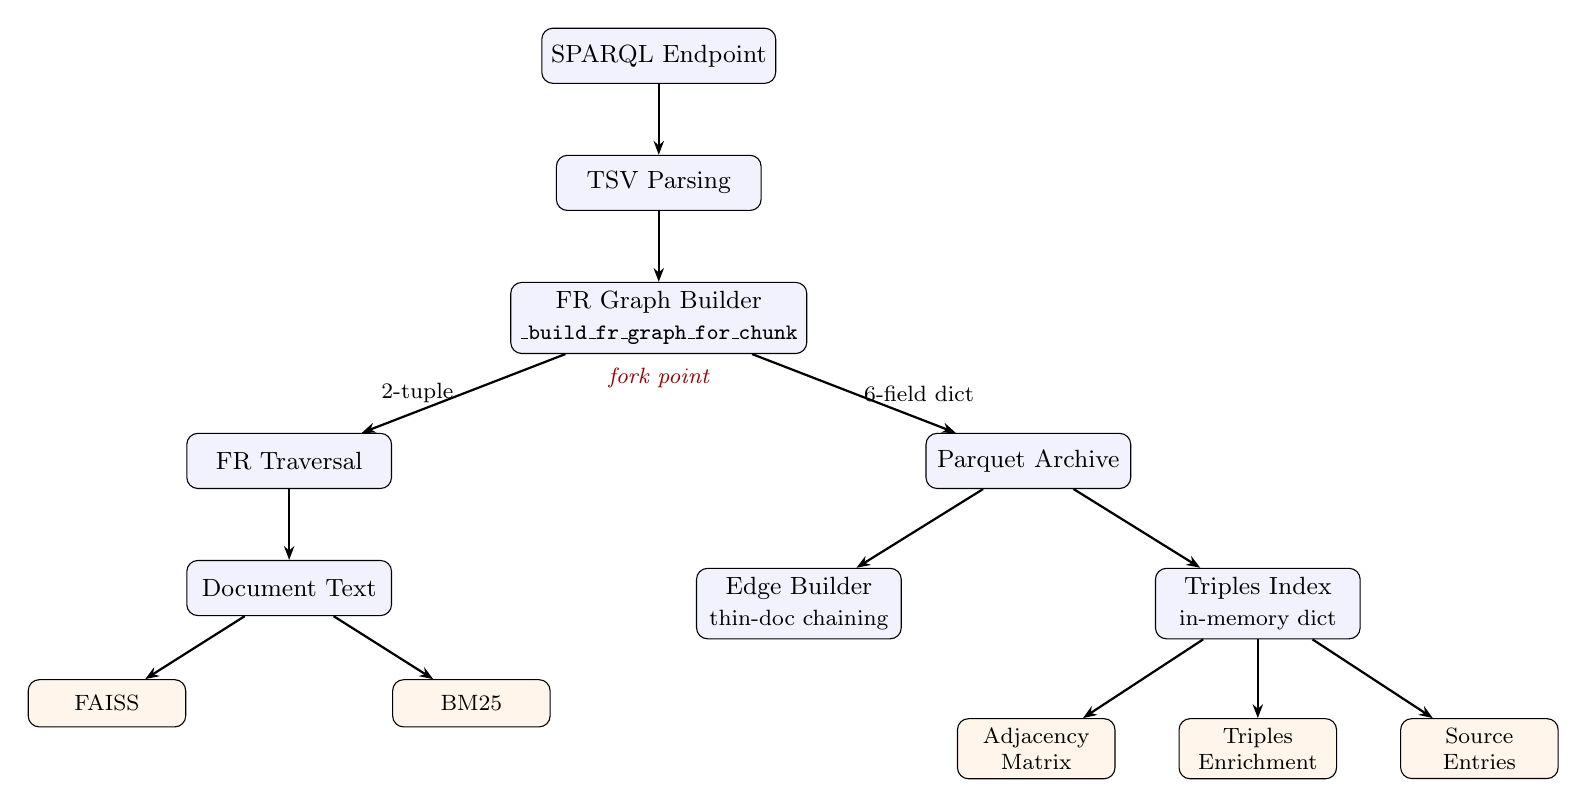
\begin{tikzpicture}[
    node distance=0.9cm and 1.8cm,
    every node/.style={font=\small},
    box/.style={draw, rounded corners, minimum width=2.6cm, minimum height=0.7cm, align=center, fill=blue!5},
    smallbox/.style={draw, rounded corners, minimum width=2.0cm, minimum height=0.6cm, align=center, fill=orange!8, font=\footnotesize},
    arr/.style={-{Stealth[length=5pt]}, thick},
  ]

  % Build-time nodes
  \node[box] (sparql) {SPARQL Endpoint};
  \node[box, below=of sparql] (tsv) {TSV Parsing};
  \node[box, below=of tsv] (fork) {FR Graph Builder\\{\footnotesize\texttt{\_build\_fr\_graph\_for\_chunk}}};

  % Left branch: FR path
  \node[box, below left=1.0cm and 1.5cm of fork] (fr) {FR Traversal};
  \node[box, below=of fr] (doc) {Document Text};
  \node[smallbox, below left=0.8cm and 0.0cm of doc] (faiss) {FAISS};
  \node[smallbox, below right=0.8cm and 0.0cm of doc] (bm25) {BM25};

  % Right branch: Parquet path
  \node[box, below right=1.0cm and 1.5cm of fork] (parquet) {Parquet Archive};
  \node[box, below left=1.0cm and 0.3cm of parquet] (edges) {Edge Builder\\{\footnotesize thin-doc chaining}};
  \node[box, below right=1.0cm and 0.3cm of parquet] (index) {Triples Index\\{\footnotesize in-memory dict}};

  % Query-time consumers
  \node[smallbox, below left=1.0cm and 0.5cm of index] (adj) {Adjacency\\Matrix};
  \node[smallbox, below=1.0cm of index] (enrich) {Triples\\Enrichment};
  \node[smallbox, below right=1.0cm and 0.5cm of index] (src) {Source\\Entries};

  % Arrows
  \draw[arr] (sparql) -- (tsv);
  \draw[arr] (tsv) -- (fork);
  \draw[arr] (fork) -- node[left, font=\footnotesize] {2-tuple} (fr);
  \draw[arr] (fork) -- node[right, font=\footnotesize] {6-field dict} (parquet);
  \draw[arr] (fr) -- (doc);
  \draw[arr] (doc) -- (faiss);
  \draw[arr] (doc) -- (bm25);
  \draw[arr] (parquet) -- (edges);
  \draw[arr] (parquet) -- (index);
  \draw[arr] (index) -- (adj);
  \draw[arr] (index) -- (enrich);
  \draw[arr] (index) -- (src);

  % Fork annotation
  \node[font=\footnotesize\itshape, text=red!60!black] at ($(fork.south)+(0,-0.3)$) {fork point};

\end{tikzpicture}
\caption{Lifecycle of an RDF triple through the \crmrag{} pipeline.
After SPARQL extraction, the triple forks into an FR traversal path (producing document text for vector indexing) and a Parquet archival path.
The archive is read twice---once at build time for graph edge construction, once at startup for the in-memory triples index---and the index serves three query-time consumers: the adjacency matrix for re-ranking, triples enrichment for the LLM prompt, and source entries for the API response.}
\label{fig:lifecycle}
\end{figure}

% ===================================================================
\section{Answering Questions: The Query Phase}
\label{sec:query}

\subsection{Query Analysis}
\label{sec:analysis}

When a user submits a question, the system begins by classifying it through an LLM call that determines three properties.
The \emph{query type} indicates whether the question targets a specific entity (\enquote{Tell me about Panagia Phorbiottisa}), requests an enumeration (\enquote{Which paintings depict saints?}), or seeks an aggregation (\enquote{How many churches are in Cyprus?}).
This classification controls the retrieval budget: specific queries retrieve 10~documents, enumerations~20, and aggregations~25.
The \emph{target categories} identify which FCs the user wants as the answer---Thing for artworks, Actor for people---and guide FC-aware filtering in later stages.
The \emph{context categories} capture FCs that are mentioned as filters or background but are not themselves the answer type; in \enquote{Which artists worked in Geneva?}, Actor is the target and Place is context.
The output of query analysis---the query type, target categories, and context categories---governs the retrieval budget and filtering decisions in all subsequent stages.

\subsection{Candidate Retrieval}
\label{sec:retrieval}

The system assembles an initial candidate pool of documents by over-retrieving---typically six times the final count---to provide sufficient material for the re-ranking stages that follow.
This pool is built through several complementary retrieval channels.

The first channel is dense retrieval via FAISS\@.
The question is embedded into a vector using the same model that embedded the documents, and FAISS returns the documents whose vectors are nearest in the embedding space, with similarity computed as $1/(1 + d_{\text{L2}})$.
The second channel is sparse retrieval via BM25.
The question is tokenized, and BM25 returns documents that share keywords with the query, catching exact-name matches that embedding similarity might miss.
If the user types \enquote{Nikitari,} BM25 finds all documents containing that exact string, regardless of how close their embeddings happen to be.

The results from these two channels are merged using Reciprocal Rank Fusion (RRF), a standard technique for combining ranked lists from different retrieval systems without requiring score normalization.
Each document's RRF score is computed as
\begin{equation}
\text{RRF}(d) = \sum_{l \in \{\text{FAISS},\,\text{BM25}\}} \frac{1}{k + \text{rank}_l(d) + 1}
\label{eq:rrf}
\end{equation}
where $k = 60$ is a smoothing constant.
Documents that rank highly in both systems receive the highest combined scores.

A parallel FC-filtered channel operates alongside the main retrieval path.
This channel restricts FAISS and BM25 results to documents whose FC matches the query's target categories, ensuring that ontologically appropriate entities are represented in the pool.
For enumeration and aggregation queries, the FC-filtered channel additionally incorporates PageRank candidates---entities with high graph centrality computed at build time from the FR discovery graph using NetworkX with a damping factor of~0.85.
These are entities that have the most FR connections to other entities in the dataset and may not appear in the embedding-based results despite their structural importance.
The FC-filtered results are merged into the main pool, with a configurable fraction of pool slots (50\% for enumerations and aggregations, 30\% for specific queries) reserved for FC-matching documents.
A final capping step limits metadata entity classes---appellations, inscriptions, linguistic objects---to at most 25\% of the pool, preventing them from crowding out substantive results.
The output of this stage is a ranked candidate pool---typically 60~documents for a specific query, 120 for an enumeration---each carrying an RRF score that reflects its combined ranking across all retrieval channels.

\subsection{Graph-Aware Re-ranking}
\label{sec:reranking}

The candidate pool is re-ranked using the knowledge graph's relational structure, not just text similarity.
For each candidate document, the system looks up its triples in the in-memory triples index and constructs an $N \times N$ adjacency matrix~$\mathbf{A}$ that captures the connectivity between candidates.
Two types of connections contribute to this matrix.
Direct one-hop edges arise when both endpoints of a triple are candidates; each such edge receives a weight reflecting the \crm{} semantic importance of the predicate (0.9 for spatial containment, 0.8 for part-whole, 0.6 for typological classification via \prop{P2\_has\_type}).
Virtual two-hop edges arise when an intermediate entity that is not itself a candidate connects two candidates; the virtual edge weight is
\begin{equation}
w_{\text{virtual}} = \frac{w_a \cdot w_b}{h}
\label{eq:virtual}
\end{equation}
where $w_a$ and $w_b$ are the weights of the two hops and $h$~is the hop count, capturing the intuition that indirect connections are weaker than direct ones but still informative.
The matrix is symmetrically normalized as $\hat{\mathbf{A}} = \mathbf{D}^{-1/2}\,\mathbf{A}\,\mathbf{D}^{-1/2}$ to prevent high-degree nodes from dominating the connectivity signal.

The final document selection proceeds greedily through a coherent subgraph extraction algorithm.
The document with the highest relevance score is selected first.
In each subsequent round, every remaining candidate~$d$ is scored as
\begin{equation}
\text{score}(d) = \alpha \cdot \text{rel}(d) + (1 - \alpha) \cdot \text{conn}(d, S) - \lambda \cdot \max_{s \in S} \cos(\mathbf{e}_d, \mathbf{e}_s)
\label{eq:subgraph}
\end{equation}
where $\text{rel}(d)$ is the normalized RRF score, $\text{conn}(d, S)$ is the average adjacency weight between~$d$ and the already-selected set~$S$, $\mathbf{e}_d$ and $\mathbf{e}_s$ are embedding vectors, $\alpha = 0.7$ balances relevance against connectivity, and $\lambda = 0.2$ is the MMR-style diversity penalty that prevents near-duplicate entities from flooding the result set.
The process continues until the desired number of documents has been selected.
The resulting set---the final output of the retrieval pipeline---consists of documents that are individually relevant to the query, mutually connected through the knowledge graph, and diverse in their content.
These selected documents, together with their triples from the in-memory index, become the input to context assembly.

A critical property of this re-ranking pipeline is that its computational cost is bounded by the candidate pool size, not by the dataset size.
A specific query produces a $60 \times 60$ adjacency matrix regardless of whether the dataset contains 286 or 866{,}000~documents.
The pool size is determined by configuration constants, making query latency predictable across datasets of any scale.

\subsection{Context Assembly and Answer Generation}
\label{sec:generation}

The selected documents from the re-ranking stage are assembled into a prompt for the language model through a structured context-building process.
Each document's natural language text is included, truncated to 5{,}000~characters to stay within model context limits.
Alongside the document text, the system appends a structured triples enrichment section.
For each retrieved document, it looks up all triples from the in-memory index, filters out schema predicates (\prop{rdf:type}, \prop{rdfs:label}, \prop{owl:inverseOf}), and formats the remainder as relationship lines.
These triples are prioritized by a four-level scheme: triples connecting two retrieved documents receive the highest priority, followed by high-value predicates (temporal, creator, location, depiction), then predicates with human-readable labels, and finally everything else.
Time-span URIs are resolved to their actual date values by following \prop{P82a} and \prop{P82b} properties in the triples index.
The total enrichment is capped at 5{,}000~characters, with per-entity budgets allocated proportionally to entity importance.

For enumeration and aggregation queries, the prompt additionally includes dataset-level statistics drawn from the aggregation index: entity class counts, FC distribution, and the top entities by PageRank.
The system prompt itself is tuned to the query type---enumeration queries receive an instruction to list all matching entities comprehensively, while aggregation queries receive an instruction to count or rank.

The language model generates an answer grounded in the assembled context.
The response is returned to the user alongside source documents, each carrying its URI, human-readable label, images (where available from Wikidata), and the structured triples that support the answer.

% ===================================================================
\section{Multi-Turn Conversation}
\label{sec:multiturn}

\crmrag{} supports multi-turn conversations in which each question can build on the previous exchange.
When a follow-up question is detected through the presence of chat history, the system employs dual retrieval: it runs the retrieval pipeline twice, once with a contextualized query that prepends the previous question and answer to the current question, and once with the raw current question alone.
The results are interleaved and deduplicated.
The contextualized pass ensures that anaphoric references (\enquote{What style is it?}) are grounded in the prior turn, while the raw pass catches cases where the added context shifts the embedding away from the user's actual intent.

Two special cases receive dedicated handling.
Pivot questions---those containing exclusion phrases such as \enquote{aside from Asinou} or \enquote{other than this church}---trigger a pattern-matching detector that strips the exclusion phrase and retrieves against the cleaned query, preventing results from being dominated by the excluded entity.
Vague follow-ups---questions dominated by stopwords and containing fewer than ten content words, such as \enquote{Tell me more} or \enquote{What about that?}---skip the raw retrieval pass entirely, since the raw query would be too generic to produce useful results.

% ===================================================================
\section{Scaling Considerations}
\label{sec:scaling}

The system is designed to operate across a wide range of dataset sizes, from small collections of a few hundred entities to institutional corpora with hundreds of thousands.
Two design choices make this possible.

First, the build phase never loads the full triple set into memory.
The Parquet archive is written incrementally through a streaming writer that stays open across chunks, and read back in batches of 500{,}000~rows.
Embeddings are cached per entity on disk, allowing the build process to be interrupted and resumed without re-embedding.
These choices mean that the build phase's memory footprint is proportional to the chunk size and batch size, not to the total dataset.

Second, the query phase's most expensive component---the adjacency matrix---operates on the candidate pool, not on the full document set.
The pool size is $k \times m$ where $k$~is the retrieval count and $m$~is a constant multiplier (default~6).
A specific query over a dataset of 866{,}000~documents produces the same $60 \times 60$ matrix as a specific query over 286~documents.
The deduplication mechanism at Parquet write time also matters for scale: because two-hop fetching causes intermediate entities to appear in multiple chunks, the hash-based dedup prevents archive bloat that would otherwise grow quadratically with the number of chunks sharing intermediaries.

% ===================================================================
\section{Summary}
\label{sec:summary}

\crmrag{} converts a \crm{} knowledge graph into a question-answering system through a pipeline with a clear separation between build-time and query-time concerns.
The build phase extracts triples from a SPARQL endpoint, traverses multi-hop FR paths to generate entity-centric natural language documents, absorbs thin vocabulary entities into their parents, embeds the documents into both dense and sparse indexes, and archives the raw triples in a structured Parquet file for query-time consumption.
The query phase classifies the user's question, retrieves an over-sized candidate pool through hybrid FAISS and BM25 retrieval with FC-aware filtering and PageRank fusion, re-ranks candidates through a graph-aware coherent subgraph selection algorithm, enriches the LLM context with priority-scored structured triples, and generates an answer grounded in the selected documents.

The central architectural insight is that the same raw triples serve three different roles at three different times.
During the build phase, they are consumed by FR traversal to produce document text and by edge building to construct the graph used for thin-document chaining.
At application startup, they are loaded from the Parquet archive into an in-memory index.
At query time, they feed the adjacency matrix for re-ranking, the triples enrichment for LLM context, and the source entries for the API response.
The Parquet archive, written incrementally and deduplicated at write time, is the single persistent store that bridges these uses---read twice during the build-startup sequence and never again thereafter.

% ===================================================================
\bibliographystyle{plain}
\begin{thebibliography}{9}

\bibitem{tzompanaki2012}
K.~Tzompanaki and M.~Doerr.
\newblock Fundamental Categories and Relationships for intuitive querying CIDOC-CRM based repositories.
\newblock \emph{Technical Report ICS-FORTH/TR-429}, Institute of Computer Science, FORTH, 2012.

\bibitem{leboeuf2023}
P.~Le~Boeuf, M.~Doerr, C.\,E.~Ore, and S.~Stead.
\newblock \emph{Definition of the CIDOC Conceptual Reference Model} (Version 7.1.3).
\newblock ICOM/CIDOC CRM Special Interest Group, 2023.

\end{thebibliography}

\end{document}
